\newpage
\section{Experimental Setup and Hyper-parameters}
\label{sec:Experimental-setup}

Our experimental setup was designed to optimize the performance of instruction fine-tuning on LLMs and to accurately assess their capabilities in legal judgment prediction and explanation tasks. We utilized two cores of NVIDIA A100-PCIE-40GB with 126GB RAM of 32 cores for instruction fine-tuning, ensuring powerful computational resources for processing and model training. In addition to the dedicated hardware, we employed a Google Colab Pro subscription having A100 Hardware accelerator for conducting inference and other experiments. This platform provided us with the necessary flexibility and scalability for our extensive experimentation.

Regarding the model training specifics, we fine-tuned the LLMs for 5 epochs. This duration was chosen to balance between adequately training the models on our \texttt{PredEx} dataset and preventing overfitting. During our experiments, we encountered a common issue with generative models – the tendency to hallucinate and repeat sentences. To address this, we implemented a post-processing step after inference. This step involved selecting the first occurrences of the decision and explanation parts from the model outputs and omitting any subsequent repetitions. This approach helped us refine the output quality, ensuring the results to be coherent and concise.

However, it is important to note that certain LLMs did not yield inference results in some cases. In such instances, we excluded those cases from our evaluation process. This decision was made to maintain the integrity and accuracy of our experimental findings, as including non-inferential results could have skewed our overall assessment of the models' performance.

Overall, our experimental setup was carefully crafted to provide a robust and reliable framework for evaluating the efficacy of instruction-tuned LLMs in the context of legal judgment prediction and explanation.

%%%%%%%%%%%%%%%%%%%%%%%%%%%%%%%%%%%

\section{Hallucination Examples}
\label{sec:Hallucination-example}

\subsection{Pre-trained vs Fine-tuned}
In the Appendix, we conduct a thorough comparison between pre-trained and fine-tuned models to demonstrate the reduction of hallucinations through our fine-tuning methods. Table \ref{tab:ca_analysis} in the Appendix presents this comparative analysis, illustrating the impact of instruction-tuning on legal judgment prediction with explanation tasks in our PredEx dataset. This section specifically focuses on how instruction-tuning can mitigate the issues of inaccuracies often found in the responses generated by pre-trained Large Language Models (LLMs).

\subsection{Zephyr-7b-beta and Gemini pro}
For a practical illustration of hallucination issues, Table \ref{zephyr-gemini-hallucination-example} in the Appendix provides examples from the Zephyr-7b-beta and Gemini Pro models. Notably, Zephyr-7b-beta sometimes produced contradictory outcomes (`accepted' and `rejected') for the same case with identical explanations. Additionally, an instance was observed where Gemini Pro produced a decision in Chinese, despite the prompt and the rest of the proceedings being in English. These examples highlight the critical need for model training and tuning specific to the dataset and task to ensure the reliability and accuracy of AI-generated legal predictions and explanations.

%%%%%%%%%%%%%%%%%%%%%%%%%%%%%%%%%%
% hallucination_table
%%%%%%%%%%%%%%%%%%%%%%%%%%%%%%%%%%

\begin{table*}[h]
\centering
\tiny
\resizebox{\textwidth}{!}{%
\begin{tabular}{|c|l|}
\hline

\textbf{Model} &
  \multicolumn{1}{c|}{\textbf{Decision and Explanation}} \\ \hline
 
Ground Truth &
  { \begin{tabular}[c]{@{}l@{}}Decsion: Accepted. Explanation: Insofar as first issue is concerned that need \\ not detain us for long as we find that the treatment given thereto by the High \\ Court is without any blemish.................................................The High Court \\ has held that it provides for only one situation where the time period can be \\ stretched, viz. where the assessment is held up (after due service of notice) \\ due to a stay order by a court of law. That covers only one eventuality, namely \\ assessment proceedings. The fact that the other periods have not been \\ mentioned leads to the inference that the delay in issuance of notice, or \\ delays in other situations have been intentionally left out, and the \\ consequence of such imperatively framed time period being breached, \\ result in invalidity of the act.\end{tabular}} \\ \hline
Zephyr-7b-beta &
  { \begin{tabular}[c]{@{}l@{}}{[}1, The appeal is likely to be allowed.{]}\\ \\ Explanation: The High Court has held that the notice issued for revising the \\ assessment list was not valid for the assessment year 1997-98 as it was \\ issued after the expiry of the assessment year. However, the notice was \\ received during the assessment year 1998-99. The Court has clarified that \\ the notice could not have been used to revise the assessment list for the \\ year 1997-98, but it was valid for the year 1998-99. Therefore, the Court is \\ likely to allow the appeal as the assessment list for the year 1998-99 was \\ validly revised.\\ \\ {[}0, The appeal is not likely to be allowed.{]}\\ \\ Explanation: The High Court has held that the notice issued for revising the \\ assessment list was not valid for the assessment year 1997-98 as it was \\ issued after the expiry of the assessment year. However, the notice was \\ received during the assessment year 1998-99. The Court has clarified that \\ the notice could not have been used to revise the assessment list for the \\ year 1997-98, but it was validly used to revise the assessment list for the \\ year 1998-99. Therefore, the appeal is not likely to be allowed as the issue \\ at hand is related to the assessment year 1997-98, for which the notice was \\ not valid.\end{tabular}} \\ \hline

Ground Truth &
  { \begin{tabular}[c]{@{}l@{}}Decision: Rejected \\ Explanation: At the outset we would like to say that we do not find any \\ substance in the contention of learned counsel for the appellant that there \\ has been any confusion of the issue or that any wrong approach has been \\ adopted by the taxing authorities, the Tribunal or the High Court.................\\ .............no deduction in respect of interest credited by the assessee to the \\ account of the college over the said sum can be allowedIn the circumstances, \\ in our view, the High Court rightly answered the questions referred to it \\ against the assessee in both the references.\end{tabular}} \\ \hline
Gemini pro &
  {\begin{tabular}[c]{@{}l@{}}Decision: \textcolor{red}{Chinese Character} \\Explanation: The High Court held that such a view was clearly sustainable \\ and observed that it is not the requirement under s. 27(iii) that the assessee \\ must further show that the borrowing of the capital was necessary for the \\ business so that if at the time of the borrowing the assessee has sufficient \\ amount of its own the deduction could not be allowed and the High Court\\  further took the view that in deciding whether a claim of interest on borrowing \\ can be allowed the fact that the assessee had ample resources its disposal \\ and need not have borrowed was not a relevant matter for consideration.\end{tabular}} \\ \hline
\end{tabular}%
}
\caption{We observe both `accept' and `reject' judgments in the response generated by Zephyr-7B-beta with the same explanation and opposite conclusion and repetitive responses. On the other hand, Gemini Pro gives responses in the Chinese language instead of English language in a few instances.}
\label{zephyr-gemini-hallucination-example}
\end{table*}
%%%%%%%%%%%%%%%%%%%%%%%%%%%%%%%%%%%%%%%%%%%%%%%%%%


%%%%%%%%%%%%%%%%%%%%%%%%%%%%
\begin{table*}[t]
\centering
\resizebox{\textwidth}{!}{%
\begin{tabular}{|c|l|l|ll}
\cline{1-3}
\textbf{Model}                                                                          & \multicolumn{1}{c|}{\textbf{Decision and Explanantion}}                  & \multicolumn{1}{c|}{\textbf{Explanation of error}}                      &  &  \\ \cline{1-3}
Ground Truth                                                                                & {\begin{tabular}[c]{@{}l@{}}Case decision: Accepted\\ Explanation:Thus, going by the principles governing the matter, propounded \\ by this Court there cannot be any doubt that the rights of the appellant-bank \\ over the pawned sugar had precedence over the claims of the Cane \\ Commissioner and that of the workmen. The High Court was, therefore, in \\ error in passing an interim order to pay parts of the proceeds to the Cane \\ Commissioner and to the Labour Commissioner for disbursal to the cane \\ growers and to the employees. There is no dispute that the sugar was \\ pledged with the appellant bank for securing a loan of the first respondent \\ and the loan had not been repaid. The goods were forcibly taken possession\\  of at the instance of the revenue recovery authority from the custody of the \\ pawnee, the appellant-bank. In view of the fact that the goods were validly \\ pawned to the appellant bank, the rights of the appellant-bank as pawnee \\ cannot be affected by the orders of the Cane Commissioner or the demands\\  made by him or the demands made on behalf of the workmen. Both the \\ Cane Commissioner and the workmen in the absence of a liquidation, stand\\  only as unsecured creditors and their rights cannot prevail over the rights of\\  the pawnee of the goods.19. We are also of the view that pending the writ \\ appeals, the High Court ought not to have passed such an interim order of \\ consequence especially in the light of the legal principles settled by this \\ Court. The order of the High Court, therefore, cannot be sustained and calls\\  for interference.\end{tabular}} & &  &  \\ \cline{1-3}
Llama-2-7B                                                                                  & { \begin{tabular}[c]{@{}l@{}}Case decision: Rejected\\ Explanation:\\ \\ The case proceedings provide several significant sentences that indicate the\\  outcome of the case will be rejected. Firstly, the court notes that the rights of\\  a pawnee over the pawned goods have precedence over the claims of a \\ secured creditor, even in the absence of a liquidation (para 15). This \\ suggests that the appellant bank's rights as a pawnee cannot be affected by\\  the orders of the Cane Commissioner or the demands made by him, even\\  though the goods were taken possession of at the instance of the revenue \\ recovery authority.\\ \\ Furthermore, the court observes that the Cane Commissioner and the\\  workmen stand only as unsecured creditors in the absence of a liquidation,\\  and their rights cannot prevail over the rights of the pawnee of the goods \\ (para 16). This implies that the appellant bank's rights as a pawnee are\\  superior to those of the Cane Commissioner and the workmen, and cannot \\ be ignored or set aside in favor of the latter.\\ \\ Finally, the court notes that the High Court's interim order was passed in \\ error, as it failed to recognize the appellant bank's rights as a pawnee \\ (para 18). This suggests that the High Court's decision will be reversed, and\\  the appellant bank's rights will be upheld.\\ \\ Based on these significant sentences in the case proceedings, it can be \\ concluded that the case will be rejected, and the appellant bank's rights as a\\  pawnee will be upheld.\end{tabular}}                                                                                & \begin{tabular}[c]{@{}l@{}}The Vanilla model incorrectly \\ categorises the sugarcane growers and\\  the workmen, represented by the Cane\\  commissioner and the Labour \\ Commissioner respectively, as "secured\\  creditors" when in actuality they are \\ "unsecured creditors" as already \\ established in the case text. This \\ hallucination is all the more apparent \\ as the model correctly identifies the \\ parties as "unsecured" creditors a few \\ lines later. Furthermore, the model \\ incorrectly places references to \\ different paragraphs of the case text,\\  i.e., para 15 and para 16. as the \\ paragraphs in question do not reflect\\  the text as purported by the model in \\ its output.\end{tabular} &  &  \\ \cline{1-3}
\begin{tabular}[c]{@{}c@{}}Llama-2-7B \\ Instruction-tuning\\ on prediction \\ with explanation\\ task\end{tabular} & \begin{tabular}[c]{@{}l@{}}Case decision: Accepted\\ Explanation:\\ \\ 18. Thus, going by the principles governing the matter, propounded by this \\ Court there cannot be any doubt that the rights of the appellant-bank over the\\  pawned sugar had precedence over the claims of the Cane Commissioner\\  and that of the workmen. The High Court was, therefore, in error in passing \\ an interim order to pay parts of the proceeds to the Cane Commissioner and\\  to the Labour Commissioner for disbursal to the cane growers and to the \\ employees. There is no dispute that the sugar was pledged with the appellant\\  bank for securing a loan of the first respondent and the loan had not been \\ repaid. The goods were forcibly taken possession of at the instance of the \\ revenue recovery authority from the custody of the pawnee, the \\ appellant-bank. In view of the fact that the goods were validly pawned to the\\  appellant bank, the rights of the appellant-bank as pawnee cannot be\\  affected by the orders of the Cane Commissioner or the demands made by\\  him or the demands made on behalf of the workmen. \textcolor{blue}{Both the Cane}\\  \textcolor{blue}{Commissioner and the workmen in the absence of a liquidation, stand} \\ \textcolor{blue}{only as unsecured creditors and their rights cannot prevail over the} \\ \textcolor{blue}{rights of the pawnee of the goods.}19. We are also of the view that pending\\  the writ appeals, the High Court ought not to have passed such an interim\\  order of consequence, especially in the light of the legal principles settled by\\  this Court. The order of the High Court, therefore, cannot be sustained and \\ calls for interference.\end{tabular}                                      & \begin{tabular}[c]{@{}l@{}}The Finetuned model accurately \\ categorises the workmen and the \\ sugarcane growers as "unsecured \\ creditors" and correctly determines that\\  the right of the pawnee (Appellant\\  Bank) will have precedence over their \\ rights to recompensation. Furthermore,\\  the finetuned model also accurately\\  states if the liquidation of the company\\  had been put into motion, the workmen\\  would THEN ONLY be considered \\ "secured creditors" in pari-passu with \\ other secured creditors.\end{tabular}&  &  \\ \cline{1-3}
\end{tabular}%
}
\caption{Comparative analysis of responses generated by Pretrained Llama-2-7B and Instruction Finetuned Llama-2-7B.}
\label{tab:ca_analysis}
\end{table*}
%%%%%%%%%%%%%%%%%%%%%%%%%
% %%%%%%%%%%%%%%%%%%%%%%%%%%%%%%%%%%%%
\begin{figure*}[h]
    \centering

    \begin{tcolorbox}[colframe=black, colback=white, boxrule=1pt, arc=0mm, outer arc=0mm]
    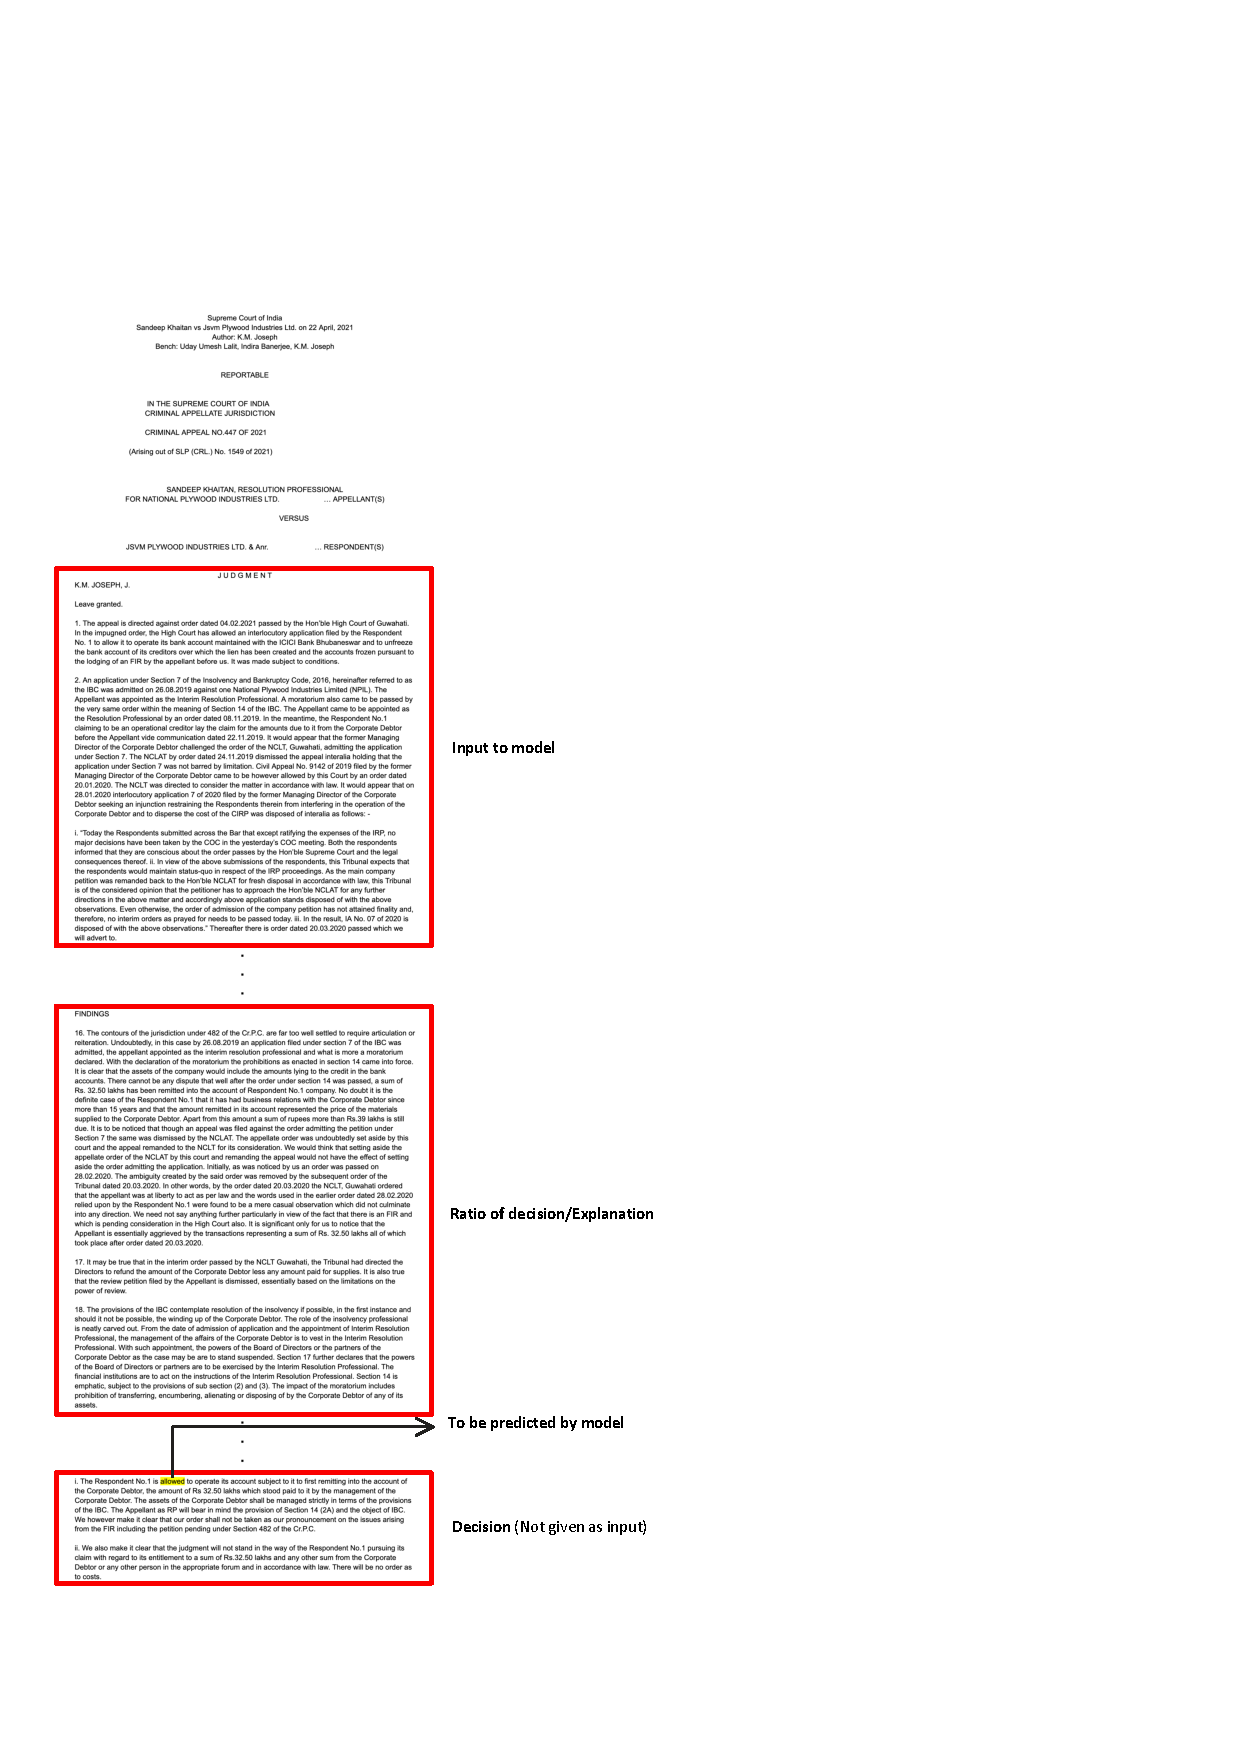
\includegraphics[trim=0.8cm 0.8cm 0.9cm 0.6cm, clip, scale=1]{images/PredEx-Case-Example.pdf}

    \end{tcolorbox}
    \caption{Annotated Example of Judicial Reasoning Extraction.}
    \label{fig:annotated-example}
\end{figure*}
% %%%%%%%%%%%%%%%%%%%%%%%%%%%%%%%%%%%%

%%%%%%%%%%%%%%%%%%%%%%%%%
% Indian Case Structure Example
%%%%%%%%%%%%%%%%%%%%%%%%%

% \section{Indian Case Structure Example}

\begin{table*}[t]
\centering
\resizebox{\textwidth}{!}{%
\begin{tabular}{|
>{}l |}
\hline
\textbf{CASE NO:} \\ \hline
Appeal (civil) 3499-3500 of 2007 \\ \hline
\textbf{PETITIONER:} \\ \hline
CENTRAL BANK OF INDIA \\ \hline
\textbf{RESPONDENT:} \\ \hline
SIRIGUPPA SUGARS \& CHEMICALS LTD. \& ORS \\ \hline
\textbf{DATE OF JUDGMENT:} \\ \hline
07/08/2007 \\ \hline
{ \textbf{BENCH:}} \\ \hline
{ TARUN CHATTERJEE \& P.K. BALASUBRAMANYAN} \\ \hline
\textbf{CASE TEXT:} \\ \hline
{ \begin{tabular}[c]{@{}l@{}}...These appeals challenge the interim order passed by the Division Bench of the High Court in a pending writ appeal, directing \\ disbursement of certain amounts realised on sale of stocks of sugar, owned by the first respondent company held under\\  pledge by the appellant--bank. The Labour Commissioner had passed an order under \textcolor{blue}{Section 33(c)} of the Industrial \\ Disputes Act against the first respondent company in respect of the dues to the workmen. The same was challenged by the \\ first respondent in the writ petition as also by others...\\ \\  ...In \textcolor{magenta}{Giles vs. Grover (1832 (131) ER 563 : 9 Bing 128)} it has been held that the Crown has no precedence over a pledgee of\\  goods. In Bank of Bihar vs. State of Bihar (supra) the principle has been recognised by this Court holding that the rights of the\\  pawnee who has parted with...\\ \\ ...There is no difference between the common law of England and the law with regard to pledge as codified. Under \\ \textcolor{blue}{Section 172} a pledge is a bailment of the goods as security for payment of a debt or  performance of a promise. \textcolor{blue}{Section 173}\\  entitles a pawnee to retain the goods pledged as security for payment of a debt and\\  under \textcolor{blue}{Section 175} he is entitled to receive from the pawner any extraordinary expenses he incurs for the preservation of the\\  goods pledged with him... \\ \\ ...In \textcolor{magenta}{State of M.P. vs. Jaura Sugar Mills Ltd. And others} (supra) dealing with the Madhya Pradesh\\ Sugar Cane (Regulation and Supply) Act, it was only held that the Cane Commissioner having power to compel the cane\\  growers to supply cane to the factory, has incidental power and is duty bound to ensure payment of the price of the\\  sugarcane supplied by the sugarcane growers...\end{tabular}} \\ \hline
\textbf{JUDGEMENT:} \\ \hline
{ \begin{tabular}[c]{@{}l@{}}...We, therefore, \textcolor{ForestGreen}{allow these appeals} and set aside the impugned order of the High Court, directing payment out of parts of the\\  sale proceeds to the Labour Commissioner and to the Cane Commissioner. \textcolor{ForestGreen}{We hold that the appellant as the pawnee, is} \\ \textcolor{ForestGreen}{entitled to the amount in satisfaction of its debt to secure which, the goods had been pawned and to appropriate the} \\ \textcolor{ForestGreen}{sale proceeds towards the debt due and only if there is surplus...}\end{tabular}} \\ \hline
\end{tabular}%
}
\caption{Example of Indian Case Structure. Sections referenced are highlighted in blue, previous judgments cited are in magenta, and the final decision is indicated in green.}
\label{case-example}
\end{table*}
%%%%%%%%%%%%%%%%%%%%%%%%%%%%%%%%%%%%%%%%%%%%%%%

%%%%%%%%%%%%%%%%%%%%%%%%%%%%%%%%%%%%%%%%%%%%%%%
\begin{table*}[h]
%\small
    \centering
    \begin{tabular}{|p{0.8\textwidth}|}
    \hline
{\bf Template 1 (prediction + explanation)}\\
\hline
   
{\bf prompt} = f``````Task: Given a Supreme Court of India case proceeding enclosed in angle brackets $<$ $>$, your task is to predict the decision of the case (with respect to the appelant) and provide an explaination for the decision.\\


{\bf Prediction}: Given a case proceeding, the task is to predict the decision 0 or 1, where the label 1 corresponds to the acceptance of the appeal/petition of the appellant/petitioner and the label 0 corresponds to the rejection of the appeal/petition of the appellant/petitioner,  Explanation: The task is to explain how you arrived at the decision by predicting important sentences that lead to the decision. \\


{\bf Context}: Answer in a consistent style as shown in the following two examples: \\


  {\bf case\_proceeding}: \# case\_proceeding example 1\\


  {\bf Prediction}: \# example 1 prediction \\


  {\bf Explanation}: \# example 1 explanation\\


  {\bf case\_proceeding}: \# case\_proceeding example 2\\


 {\bf  Prediction}: \# example 2 prediction\\


 {\bf Explanation}: \# example 2 explanation\\


{\bf Instructions}: Learn from the above given two examples and perform the task for the following case proceeding. \\


case\_proceeding: $<$\{case\_proceeding\}$>$\\


Format your output in list format: [prediction, explanation]''''''\\

\hline
    {\bf Template 2 (prediction only)}\\
    \hline
   
{\bf prompt} = f``````Task: Given a Supreme Court of India case proceeding enclosed in angle brackets $<$ $>$, your task is to predict the decision of the case (with respect to the appellant).\\


{\bf Prediction}: Given a case proceeding, the task is to predict the decision 0 or 1, where the label 1 corresponds to the acceptance of the appeal/petition of the appellant/petitioner and the label 0 corresponds to the rejection of the appeal/petition of the appellant/petitioner \\


{\bf Context}: Answer in a consistent style as shown in the following two examples: \\


  {\bf case\_proceeding}: \# case\_proceeding example 1\\


  {\bf Prediction}: \# example 1 prediction \\


 


  {\bf case\_proceeding}: \# case\_proceeding example 2\\


  {\bf Prediction}: \# example 2 prediction\\


 


{\bf Instructions}: Learn from the above given two examples and perform the task for the following case proceeding. \\


{\bf case\_proceeding}: $<$\{case\_proceeding\}$>$\\


Give the output predicted case decision as either 0 or 1.''''''\\

\hline

    \end{tabular}
    \caption{Prompts for Judgment Prediction taken from \cite{vats-etal-2023-llms}.}
    \label{tab:judgment_prediction_prompts_few}
\end{table*}
%%%%%%%%%%%%%%%%%%%%%%%%%%%%%%%%%%%%%%%%%%%%%%%

%%%%%%%%%%%%%%%%%%%%%%%%%%%%%%%%%%%%%%%%%%%%%%%
\begin{table*}[h]
%\small
    \centering
    \begin{tabular}{|p{0.8\textwidth}|}
    \hline
    {\bf Template 3 (prediction only)}\\
    \hline
   
{\bf prompt} = f``````
\#\#\# {\bf Instructions}: Analyze the case proceeding and predict whether the appeal/petition will be rejected (0) or accepted (1). \\

\#\#\# \textbf{Input}: $<$\{case\_proceeding\}$>$\\


\#\#\# Response:
  ''''''\\
\hline
    {\bf Template 4 (prediction with explanation)}\\
    \hline
   
{\bf prompt} = f``````
\#\#\# {\bf Instructions}: Analyze the case proceeding and predict whether the appeal/petition will be accepted (1) or rejected (0), and subsequently provide an explanation behind this prediction with important textual evidence from the case. \\

\#\#\# \textbf{Input}: $<$\{case\_proceeding\}$>$\\


\#\#\# Response:
  ''''''\\
\hline


    \end{tabular}
    \caption{Prompts for Judgment Prediction used for instruction fine-tuned models. Instructions were randomly chosen from Table \ref{Instruction-sets}.}
    \label{tab:judgment_prediction_prompts_zero}
\end{table*}
%%%%%%%%%%%%%%%%%%%%%%%%%%%%%%%%%%%%%%%%%%%%%%%

%%%%%%%%%%%%%%%%%%%%%%%%%%%%%%%
\begin{table*}[h]
\centering
\resizebox{0.95\textwidth}{!}{%
\tiny
\begin{tabular}{|cl|}
\hline
\multicolumn{2}{|c|}{\textbf{\textcolor{blue}{Instruction sets for Predicting the Decision}}} \\ \hline
\multicolumn{1}{|c|}{1} &
  Analyze the case proceeding and predict whether the appeal/petition will be accepted (1) or rejected (0). \\ \hline
\multicolumn{1}{|c|}{2} &
  \begin{tabular}[c]{@{}l@{}}Based on the information in the case proceeding, determine the likely outcome: acceptance (1) or \\ rejection (0) of the appellant/petitioner's case.\end{tabular} \\ \hline
\multicolumn{1}{|c|}{3} &
  Review the case details and predict the decision: will the court accept (1) or deny (0) the appeal/petition? \\ \hline
\multicolumn{1}{|c|}{4} &
  \begin{tabular}[c]{@{}l@{}}Considering the arguments and evidence in case proceeding, predict the verdict: is it more likely to be in \\ favor (1) or against (0) the appellant?\end{tabular} \\ \hline
\multicolumn{1}{|c|}{5} &
  \begin{tabular}[c]{@{}l@{}}Examine the details of the case proceeding and forecast if the appeal/petition stands a chance of being \\ upheld (1) or dismissed (0).\end{tabular} \\ \hline
\multicolumn{1}{|c|}{6} &
  \begin{tabular}[c]{@{}l@{}}Assess the case proceedings and provide a prediction: is the court likely to rule in favor of (1) or against (0)\\ the appellant/petitioner?\end{tabular} \\ \hline
\multicolumn{1}{|c|}{7} &
  \begin{tabular}[c]{@{}l@{}}Interpret the case information and speculate on the court's decision: acceptance (1) or rejection (0) of the \\ presented appeal.\end{tabular} \\ \hline
\multicolumn{1}{|c|}{8} &
  \begin{tabular}[c]{@{}l@{}}Given the specifics of the case proceeding, anticipate the court's ruling: will it favor (1) or oppose (0) the \\ appellant’s request?\end{tabular} \\ \hline
\multicolumn{1}{|c|}{9} &
  \begin{tabular}[c]{@{}l@{}}Scrutinize the evidence and arguments in the case proceeding to predict the court's decision: will the appeal\\  be granted (1) or denied (0)?\end{tabular} \\ \hline
\multicolumn{1}{|c|}{10} &
  \begin{tabular}[c]{@{}l@{}}Analyze the legal arguments presented and estimate the likelihood of the court accepting (1) or rejecting (0) \\ the petition.\end{tabular} \\ \hline
\multicolumn{1}{|c|}{11} &
  \begin{tabular}[c]{@{}l@{}}From the information provided in the case proceeding, infer whether the court's decision will be positive (1) \\ or negative (0) for the appellant.\end{tabular} \\ \hline
\multicolumn{1}{|c|}{12} &
  \begin{tabular}[c]{@{}l@{}}Evaluate the arguments and evidence in the case and predict the verdict: is an acceptance (1) or rejection\\ (0) of the appeal more probable?\end{tabular} \\ \hline
\multicolumn{1}{|c|}{13} &
  \begin{tabular}[c]{@{}l@{}}Delve into the case proceeding and predict the outcome: is the judgment expected to be in support (1) or \\ in denial (0) of the appeal?\end{tabular} \\ \hline
\multicolumn{1}{|c|}{14} &
  \begin{tabular}[c]{@{}l@{}}Using the case data, forecast whether the court is likely to side with (1) or against (0) the \\ appellant/petitioner.\end{tabular} \\ \hline
\multicolumn{1}{|c|}{15} &
  \begin{tabular}[c]{@{}l@{}}Examine the case narrative and anticipate the court's decision: will it result in an approval (1) or \\ disapproval (0) of the appeal?\end{tabular} \\ \hline
\multicolumn{1}{|c|}{16} &
  \begin{tabular}[c]{@{}l@{}}Based on the legal narrative and evidentiary details in the case proceeding, predict the court's stance: \\ favorable (1) or unfavorable (0) to the appellant.\end{tabular} \\ \hline
\multicolumn{2}{|c|}{\textbf{\textcolor{blue}{Instruction sets for Integrated Approach for Prediction and Explanation}}} \\ \hline
\multicolumn{1}{|c|}{1} &
  \begin{tabular}[c]{@{}l@{}}First, predict whether the appeal in case proceeding will be accepted (1) or not (0), and then explain the \\ decision by identifying crucial sentences from the document.\end{tabular} \\ \hline
\multicolumn{1}{|c|}{2} &
  \begin{tabular}[c]{@{}l@{}}Determine the likely decision of the case (acceptance (1) or rejection (0)) and follow up with an \\ explanation highlighting key sentences that support this prediction.\end{tabular} \\ \hline
\multicolumn{1}{|c|}{3} &
  \begin{tabular}[c]{@{}l@{}}Predict the outcome of the case proceeding (1 for acceptance, 0 for rejection) and subsequently provide an\\  explanation based on significant sentences in the proceeding.\end{tabular} \\ \hline
\multicolumn{1}{|c|}{4} &
  \begin{tabular}[c]{@{}l@{}}Evaluate the case proceeding to forecast the court's decision (1 for yes, 0 for no), and elucidate the \\ reasoning behind this prediction with important textual evidence from the case.\end{tabular} \\ \hline
\multicolumn{1}{|c|}{5} &
  \begin{tabular}[c]{@{}l@{}}Ascertain if the court will uphold (1) or dismiss (0) the appeal in the case proceeding, and then clarify \\ this prediction by discussing critical sentences from the text.\end{tabular} \\ \hline
\multicolumn{1}{|c|}{6} &
  \begin{tabular}[c]{@{}l@{}}Judge the probable resolution of the case (approval (1) or disapproval (0)), and elaborate on this forecast\\  by extracting and interpreting significant sentences from the proceeding.\end{tabular} \\ \hline
\multicolumn{1}{|c|}{7} &
  \begin{tabular}[c]{@{}l@{}}Forecast the likely verdict of the case (granting (1) or denying (0) the appeal) and then rationalize your \\ prediction by pinpointing and explaining pivotal sentences in the case document.\end{tabular} \\ \hline
\multicolumn{1}{|c|}{8} &
  \begin{tabular}[c]{@{}l@{}}Assess the case to predict the court's ruling (favorably (1) or unfavorably (0)), and then expound on \\ this prediction by highlighting and analyzing key textual elements from the proceeding.\end{tabular} \\ \hline
\multicolumn{1}{|c|}{9} &
  \begin{tabular}[c]{@{}l@{}}Decide if the appeal in the case proceeding is more likely to be successful (1) or unsuccessful (0), and \\ then justify your decision by focusing on essential sentences in the document.\end{tabular} \\ \hline
\multicolumn{1}{|c|}{10} &
  \begin{tabular}[c]{@{}l@{}}Conjecture the end result of the case (acceptance (1) or non-acceptance (0) of the appeal), followed by \\ a detailed explanation using crucial sentences from the case proceeding.\end{tabular} \\ \hline
\multicolumn{1}{|c|}{11} &
  \begin{tabular}[c]{@{}l@{}}Predict whether the case will result in an affirmative (1) or negative (0) decision for the appeal, and then \\ provide a thorough explanation using key sentences to support your prediction.\end{tabular} \\ \hline
\multicolumn{1}{|c|}{12} &
  \begin{tabular}[c]{@{}l@{}}Estimate the outcome of the case (positive (1) or negative (0) for the appellant) and then give a reasoned \\ explanation by examining important sentences within the case documentation.\end{tabular} \\ \hline
\multicolumn{1}{|c|}{13} &
  \begin{tabular}[c]{@{}l@{}}Project the court's decision (favor (1) or against (0) the appeal) based on the case proceeding, and \\ subsequently give an in-depth explanation by analyzing relevant sentences from the document.\end{tabular} \\ \hline
\multicolumn{1}{|c|}{14} &
  \begin{tabular}[c]{@{}l@{}}Make a prediction on the court's ruling (acceptance (1) or rejection (0) of the petition), and then dissect \\ the proceeding to provide a detailed explanation using key textual passages.\end{tabular} \\ \hline
\multicolumn{1}{|c|}{15} &
  \begin{tabular}[c]{@{}l@{}}Speculate on the likely judgment (yes (1) or no (0) to the appeal) and then delve into the case proceeding \\ to elucidate your prediction, focusing on critical sentences.\end{tabular} \\ \hline
\multicolumn{1}{|c|}{16} &
  \begin{tabular}[c]{@{}l@{}}Hypothesize the court's verdict (affirmation (1) or negation (0) of the appeal), and then clarify this \\ hypothesis by interpreting significant sentences from the case proceeding.\end{tabular} \\ \hline
\end{tabular}%
}
% \caption{Instruction set examples}
 \caption{Instruction Sets for Predicting Legal Decisions and Providing Explanations.}
\label{Instruction-sets}
\end{table*}
%%%%%%%%%%%%%%%%%%%%%%%%%%%%%%%%%%%%%%%%%%%%%%%
